\documentclass[a4paper]{article}

%% Language and font encodings
\usepackage[english]{babel}
\usepackage[utf8x]{inputenc}
\usepackage[T1]{fontenc}

%% Sets page size and margins
\usepackage[a4paper,top=3cm,bottom=2cm,left=3cm,right=3cm,marginparwidth=1.75cm]{geometry}

%% Useful packages
\usepackage{amsmath}
\usepackage[table,xcdraw]{xcolor}
\usepackage{tabularx,booktabs}
\usepackage{graphicx}
\usepackage[colorinlistoftodos]{todonotes}
\usepackage[colorlinks=true, allcolors=blue]{hyperref}
\usepackage{amsmath}
\usepackage{tikz}
\usepackage{tkz-tab}
\usepackage{caption}
\usepackage{latexsym}
\usepackage{amssymb}
\usepackage{amsmath}
\usepackage{subcaption}
\usepackage{mathtools}
\usepackage{multirow}
\usepackage{listings}
\usepackage{color}
\usepackage{epsfig}
\usepackage{epstopdf}
\usepackage{soul}

%% Useful packages
\usepackage[table,xcdraw]{xcolor}
\usepackage{tabularx,booktabs}
\newcolumntype{C}{>{\centering\arraybackslash}X} % centered version of "X" type
\newcolumntype{b}{X}
\newcolumntype{s}{>{\hsize=.5\hsize}X}
\newcolumntype{v}{>{\hsize=.3\hsize}X}

\definecolor{mygreen}{rgb}{0,0.6,0}
\definecolor{mygray}{rgb}{0.5,0.5,0.5}
\definecolor{mymauve}{rgb}{0.58,0,0.82}


\lstdefinestyle{customc}{
  belowcaptionskip=1\baselineskip,
  breaklines=true,
  frame=L,
  xleftmargin=\parindent,
  language=C,
  showstringspaces=false,
  basicstyle=\footnotesize\ttfamily,
  keywordstyle=\bfseries\color{green!40!black},
  commentstyle=\itshape\color{purple!40!black},
  identifierstyle=\color{blue},
  stringstyle=\color{orange},
}

\lstdefinestyle{customasm}{
  belowcaptionskip=1\baselineskip,
  frame=L,
  xleftmargin=\parindent,
  language=[x86masm]Assembler,
  basicstyle=\footnotesize\ttfamily,
  commentstyle=\itshape\color{purple!40!black},
}

\lstset{escapechar=@,style=customc}

\usetikzlibrary{automata,arrows,positioning,calc}
\usetikzlibrary{shapes,snakes}

% Commands for commenting in inside the text content
\newcommand{\sergio}[1]{\textcolor{brown}{#1}}
\newcommand{\sergiost}[1]{\textcolor{brown}{\st{#1}}}
\newcommand{\franky}[1]{\textcolor{red}{#1}}


%%% TITLE
\title{Komondor User's Guide}
\author{Sergio Barrachina-Mu\~noz and Francesc Wilhelmi}

\begin{document}
\maketitle

\tableofcontents

\listoffigures

\listoftables

%%%%%%%%%%%%%%%
% 1. INTRODUCTION
%%%%%%%%%%%%%%%
\section{Introduction}
\label{section:introduction}
	Komondor \cite{barrachina2017komondor} is an event-based simulator based on COST \cite{chen2002reusing}, and which is mostly intended to reproduce the novel techniques included in the IEEE 802.11ax-2019 amendment \cite{tgax2017draft}.
	
	In this document, we aim to illustrate the installation and execution procedures that must be carried out to successfully perform Komondor simulations. For more detailed information about what is implemented in Komondor, please refer to \href{https://github.com/wn-upf/Komondor/blob/master/Documentation/Tutorial/LaTeX\%20files/komondor_technical_report.pdf}{this} document.


\section{Installation}

\section{Execution}

\section{Development Notes}


%%%%%%%%%%%%%%%
% TUTORIAL
%%%%%%%%%%%%%%%
\section{Tutorial and Development Notes}
\label{section:tutorial_and_development_notes}
	In this Section we provide a brief tutorial to encourage researchers and other practitioners to use the Komondor simulator for their own experiments, and even to participate in the project. 
	%%% Brief tutorial
	\subsection{Brief Tutorial}
	\label{section:brief_tutorial}
		Komondor is composed by several modules that allow performing simulations with a high degree of freedom. Here we provide some details on the most important modules, as well as on their practical execution. Figure \ref{fig:komondor_flowchart} summarizes the main operations carried out by Komondor.
		\begin{figure}[h!]
			\centering
			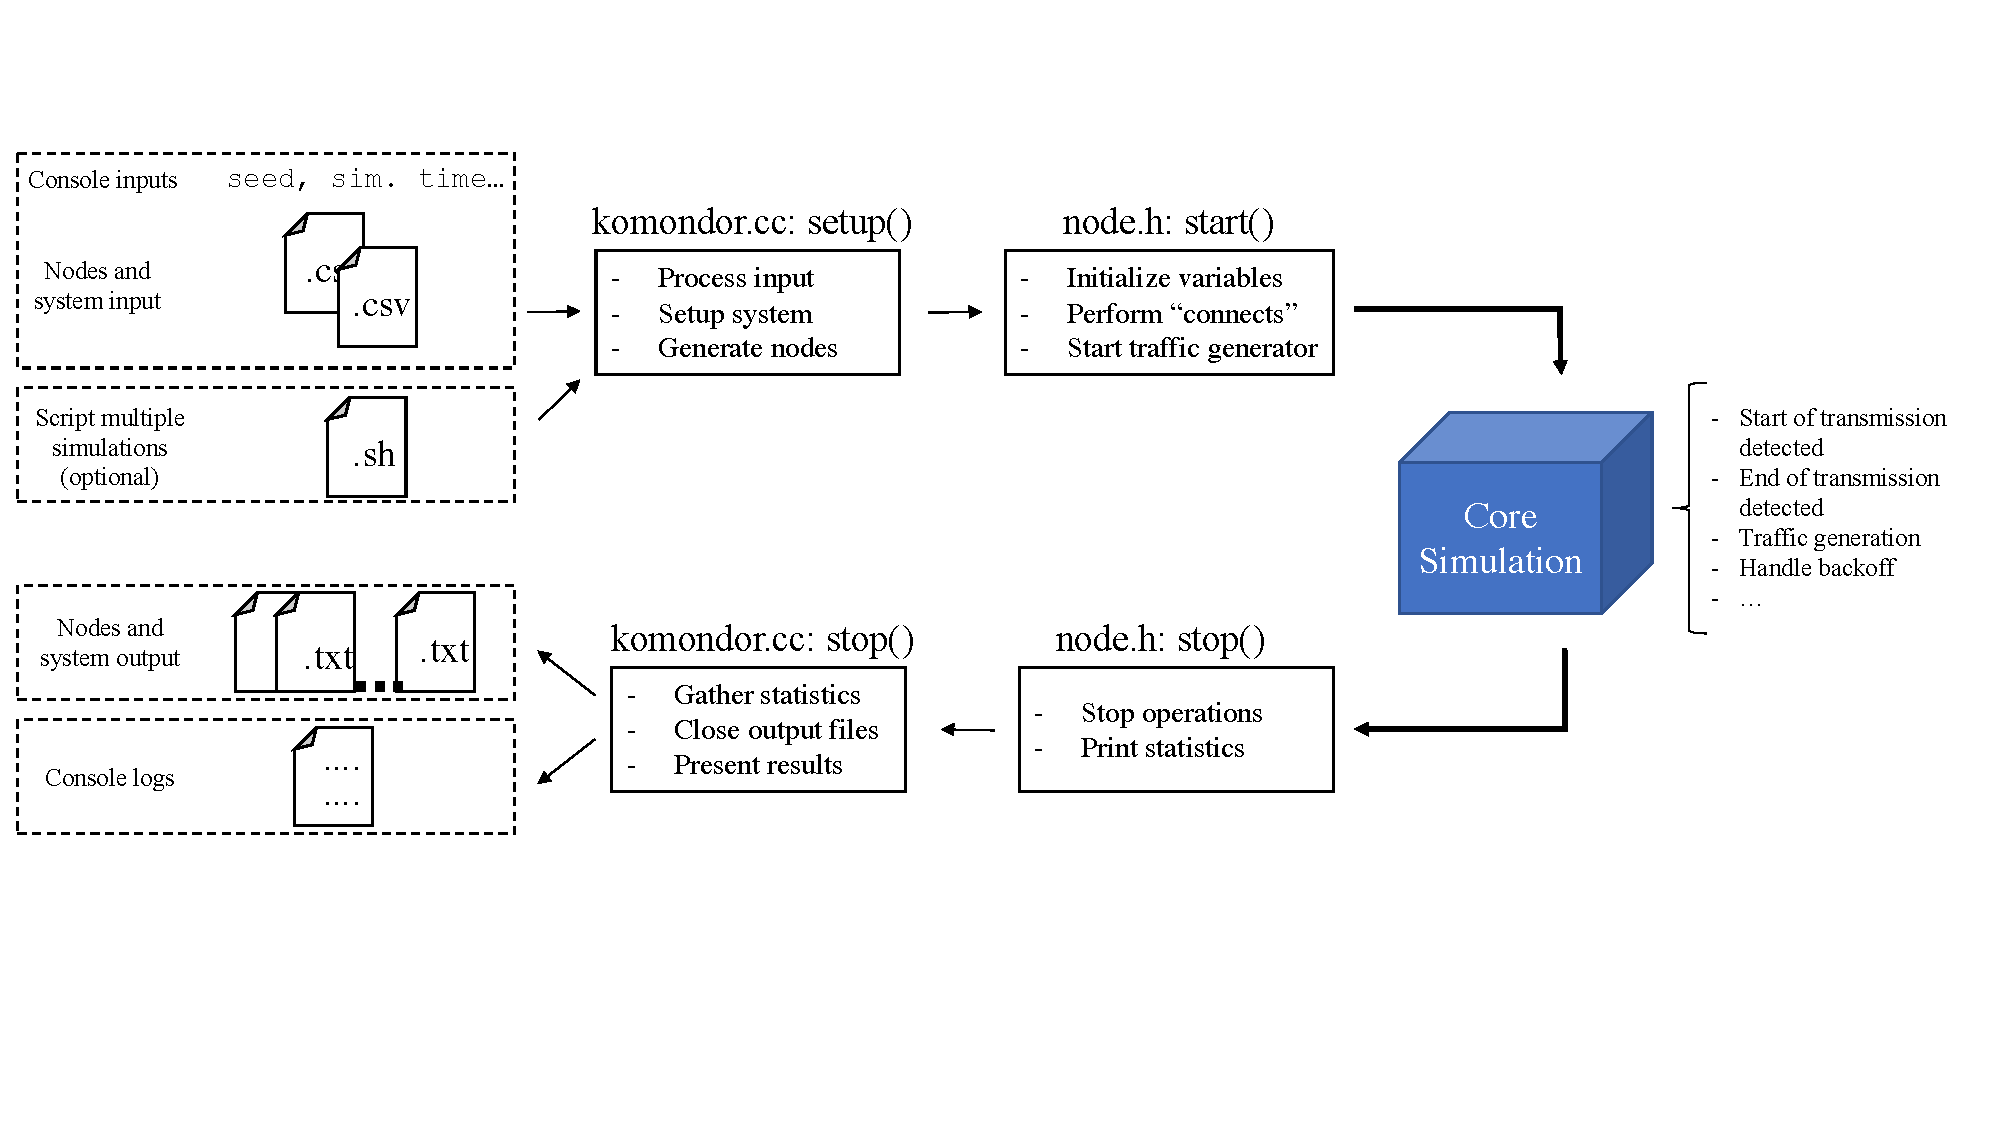
\epsfig{file=images/komondor_flowchart, width=15cm}
			\caption{Komondor flowchart}
			\label{fig:komondor_flowchart}
		\end{figure}		
		
		As shown, Komondor receives a set of inputs (nodes information, simulation time, etc.) and initializes the main module, which is in charge of generating the network and gathering useful information regarding the simulation. During the core simulation, nodes interact among each other by sending packets, so that DCF operation is implemented for accessing to the channel. Finally, when the simulation runs out, a set of outputs are generated in order to shed some light on the network performance.
		
		% Project organization
		\subsubsection{Files Organization}
		\label{section:files}		
		To properly understand the Komondor's operation, it is important to know how the project is organized, which allows obtaining a broader vision of the different modules that constitute it. The code is organized as follows:
		\begin{itemize}
			\item \textbf{COST libraries}: constitute the Komondor's primitive operation. 
			\item \textbf{Main}: contains the two core files (\texttt{komondor.cc} and \texttt{node.h}), which are in charge of orchestrating all the simulation. In addition, here we find the inputs and the file that compiles the libraries for executing the code (\texttt{build\_local}).
			\item \textbf{Methods}: by following clean architecture guidelines, independent methods used by both \texttt{komondor.cc} and \texttt{node.h} files are contained in the methods folder. Several libraries are provided according to the nature of their functions. For instance, \texttt{backoff\_methods.h} contains methods to handle the backoff operation in DCF.
			\item \textbf{Structures}: the Komondor simulator considers four main header files to carry out its operation. The first one is \texttt{wlan.h}, which defines the main characteristics of a WLAN (WLAN id, list of associated STAs, etc.). Furthermore, the \texttt{notification.h} object allows to exchange packets between devices. Finally, \texttt{logger.h} and \texttt{logical\_nack.h} are used for auxiliary purposes, which are displaying logs and notifying packet losses causes, respectively.
			\item \textbf{List of macros}: all the static parameters (e.g., constants) are contained in the \texttt{list\_of\_macros.h} file. 		
			\item \textbf{Input}: contains the input files that allow building the simulation environment.
			\item \textbf{Output}: contains the data generated by Komondor as a result of a given simulation.	
		\end{itemize}
		
		% Compilation & Execution
		\subsubsection{Compilation and Execution}
		\label{section:compilation_execution}
		To compile and execute Komondor, the following instructions must be followed\footnote{A GNU-based OS is assumed to be used for simulations, including basic compilation programs such as \emph{gcc}.}:
		\begin{enumerate}
			\item Set the .csv input files (further defined in Section \ref{section:input_files})
			\item Access to the \textit{KomondorSimulator} directory
		    \item Execute ".build\_local". This file contains the instructions for compiling the Komondor code. It has been updated to enable debugging with Valgrind\footnote{Valgrind is a programming tool for memory debugging, memory leak detection, and profiling. Valgrind main website: \url{http://valgrind.org/}}.
		    \item Execute \textit{./KomondorSimulator arg\_1 arg\_2 ... arg\_n}, where \textit{arg\_i} is the $i_{\text{th}}$ input argument:
		    	\begin{itemize}		            
		            \item \textit{arg\_1} (INPUT\_FILE\_SYSTEM\_CONFIGURATION): file containing system information (e.g., number of channels available, traffic model, etc.). The file must be a .csv with semicolons as separators.
		            \item \textit{arg\_2} (INPUT\_FILE\_NODES): file containing nodes information (e.g., position, channels allowed, etc.).The file must be a .csv with semicolons as separators.
		            \item \textit{arg\_3} (OUTPUT\_FILE\_LOGS): path to the output file to which write results at the end of the execution (if the file does not exist, the system will create it).
		            \item \textit{arg\_4} (FLAG\_SAVE\_SYSTEM\_LOGS): flag to indicate whether to save the system logs into a file (1) or not (0).\footnote{Major increases in the execution time may occur if nodes logging is activated. E.g., for a simulation of 4 nodes, simulating 1000 seconds takes 1.127 s and 15.672 s when not logging and when doing so, respectively.}
		            \item \textit{arg\_5} (FLAG\_SAVE\_NODE\_LOGS): flag to indicate whether to save the nodes logs into separate files (1) or not (0). If this flag is activated, one file per node will be created.
		            \item \textit{arg\_6} (FLAG\_PRINT\_SYSTEM\_LOGS): flag to indicate whether to print the system logs (1) or not (0).
		            \item \textit{arg\_7} (FLAG\_PRINT\_NODE\_LOGS): flag to indicate whether to print the nodes logs (1) or not (0).
		            \item \textit{arg\_8} (SIM\_TIME): simulation time in seconds.
		            \item \textit{arg\_9} (SEED): random seed for the experiments.
				\end{itemize}
		    \item Collect the results either in the output files or in the console.
		\end{enumerate}
	
		\textbf{NOTE}: in case that the user does not have permissions to execute some of the files, grant them by introducing the following command in the target folder: \texttt{\$ chmod -R 777 *}.
		
		% Input
		\subsubsection{Input files}
		\label{section:input_files}	
		To define the simulation environment, the Komondor simulator relies in the following two types of input files:
		\begin{itemize}
			\item \textbf{System input:} defines global input parameters such as the number of basic channels considered or the propagation models. System input parameters are defined in Table \ref{table:system_parameters}.
			\item \textbf{Nodes input:} defines specific nodes' characteristics such as type, location, or implementing features (e.g., DCB policy). There are two ways of generating nodes, which is indicated in the file name. 
			
			\begin{itemize}
				\item In case of including the keyword \emph{nodes}, all the devices (both APs and STAs) must be introduced and described.
				\item Otherwise, if including the keyword \emph{aps}, only the APs are defined, so that a set of STAs is randomly generated under certain introduced parameters (e.g., minimum/maximum number of STAs, maximum distance between APs and STA).\footnote{The usage of APs input files is discouraged to the lack of maintenance.}
			\end{itemize}  
		
			As a final remark, in order to ensure a proper execution, it is mandatory to introduce an input file with a list of nodes ordered by \textit{node\_id} and starting with \textit{node\_id} = 0 (it is a requirement for the array responsible of storing the power perceived by each node). Table \ref{table:nodes_parameters} describes the Nodes input parameters for both \emph{nodes} and \emph{aps} files. 
			
		\end{itemize}		
	
		

		%  System input parameters	
		\begin{table}[h!]
			\centering
			\begin{tabular}{|c|c|l|}
				\hline
				\textbf{Parameter} & \textbf{Type} & \multicolumn{1}{c|}{\textbf{Description}} \\ \hline
				num\_channels & int & \begin{tabular}[c]{@{}l@{}}Maximum number of frequency channels \\ in the system\end{tabular} \\ \hline
				basic\_channel\_bandwidth & int & Bandwidth for each channel {[}MHz{]} \\ \hline
				pdf\_backoff & int & PDF to compute the backoff () \\ \hline
				pdf\_tx\_time & int & PDF to compute the tx time () \\ \hline
				packet\_length & int & Length of data packets {[}bits{]} \\ \hline
				ack\_length & int & Length of ACK packets {[}bits{]} \\ \hline
				num\_packets\_aggregated & int & Number of packets aggregated per transmission \\ \hline
				path\_loss\_model & int & \begin{tabular}[c]{@{}l@{}}Path-loss model (0: FSPL, 1: Hata, \\ 2: Indoor 1, 3: Indoor 2, 4: TGax scenario 1)\end{tabular} \\ \hline
				capture\_effect & int & Capture Effect Threshold {[}dB{]} \\ \hline
				noise\_level & int & Floor noise level {[}dBm{]} \\ \hline
				adjacent\_channel\_model & int & \begin{tabular}[c]{@{}l@{}}Co-channel interference model \\ (0: without adjacent interference,\\ 1: contiguous adjacent interference, \\ 2: complete adjacent interference)\end{tabular} \\ \hline
				collisions\_model & int & Collisions model (reserved) \\ \hline
				SIFS & int & SIFS period {[}$\mu$s{]} \\ \hline
				constant\_PER & int & Defines a constant Packet Error Rate \\ \hline
				traffic\_model & int & \begin{tabular}[c]{@{}l@{}}Traffic model (0: full buffer, 1: Poisson distr., \\ 2: deterministic distr.)\end{tabular} \\ \hline
				backoff\_type & int & Type of backoff (discrete: 0, continuous: 1) \\ \hline
				rts\_length & int & Length of RTS packets {[}bits{]} \\ \hline
				cts\_length & int & Length of CTS packets {[}bits{]} \\ \hline
				cw\_adaptation & bool & For activating CW adaptation \\ \hline
				pifs\_activated & bool & For activating PIFS \\ \hline
			\end{tabular}
			\caption{System input parameters description}
			\label{table:system_parameters}
		\end{table}
		
		% Nodes input parameters		
		\begin{table}[h!]
			\centering
			\begin{tabular}{|c|c|c|l|}
				\hline
				\textbf{Parameter} & \textbf{Type} & \textbf{Nodes or APs} & \multicolumn{1}{c|}{\textbf{Description}} \\ \hline
				node\_code & String & nodes & Code assigned to the node \\ \hline
				node\_type & int & nodes & Type of node (0: AP, 1: STA) \\ \hline
				wlan\_code & String & both & Code assigned to the WLAN \\ \hline
				destination\_id & int & nodes & \begin{tabular}[c]{@{}l@{}}To specify the ID of the destination \\ (packets would be only sent to that devices).\\ Setting it to -1 indicates random destination.\end{tabular} \\ \hline
				min\_sta\_number & int & aps & Minimum number of associated STAs \\ \hline
				max\_sta\_number & int & aps & Maximum number of associated STAs \\ \hline
				max\_distance\_sta & int & aps & Maximum distance of associated STAs \\ \hline
				x & int & both & X location {[}m{]} \\ \hline
				y & int & both & Y location {[}m{]} \\ \hline
				z & int & both & Z location {[}m{]} \\ \hline
				primary\_channel & int & both & Primary channel \\ \hline
				min\_channel\_allowed & int & both & Left channel in range \\ \hline
				max\_channel\_allowed & int & both & Right channel in range \\ \hline
				cw & int & both & Fixed CW \\ \hline
				cw\_stage & int & both & Initial CW stage (for CW adaptation) \\ \hline
				tpc\_min & int & both & Minimum transmit power allowed {[}dBm{]} \\ \hline
				tpc\_default & int & both & Default transmit power allowed {[}dBm{]} \\ \hline
				tpc\_max & int & both & Maximum transmit power allowed {[}dBm{]} \\ \hline
				cca\_min & double & both & Minimum CCA allowed {[}dBm{]} \\ \hline
				cca\_default & double & both & Default CCA allowed {[}dBm{]} \\ \hline
				cca\_max & double & both & Maximum CCA allowed {[}dBm{]} \\ \hline
				tx\_antenna\_gain & int & both & Gain of the tx antenna {[}dB{]} \\ \hline
				rx\_antenna\_gain & int & both & Gain of the rx antenna {[}dB{]} \\ \hline
				channel\_bonding\_model & int & both & \begin{tabular}[c]{@{}l@{}}Channel bonding model (0: only primary, \\ 1: SCB, 2: SCB log2, 3: always max, \\ 4: always max log2, 5: always max log2 MCS,\\ 6: uniform probability log2)\end{tabular} \\ \hline
				modulation\_default & int & both & \begin{tabular}[c]{@{}l@{}}Modulation set by default \\ (0 to use dynamic MCS)\end{tabular} \\ \hline
				central\_freq & int & both & Frequency band used (2,4 or 5 GHz) \\ \hline
				lambda & float & both & Packets transmission rate {[}packets/s{]} \\ \hline
				ieee\_protocol & int & both & IEEE protocol used \\ \hline
			\end{tabular}
			\caption{Nodes input parameters description}
			\label{table:nodes_parameters}
		\end{table}
		
		% Input scripts
		\subsubsection{Input scripts}
		\label{section:input_scripts}	
		In order to facilitate users work, we provide a set of scripts that allow performing several simulations at once, which is useful to avoid processing different output files. Such sample scripts can be found in the ``scripts multiple executions" folder, which perform the following operations:
		\begin{itemize}
			\item \emph{multiple\_inputs\_script.sh}: processes all the input files contained in ./input/script\_input\_files and generates a simulation for each one. 
			\item \emph{multiple\_inputs\_script\_several\_seeds.sh}: in addition to process multiple inputs, generates different seeds for each simulation.
		\end{itemize}
		
		Similar procedures can be implemented to extend the current provided functionalities, such as reading multiple system inputs or generating specific output reports.
		
		% Output
		\subsubsection{Output files}
		\label{section:output_files}	
		A lot of effort has been put on the output generation, since it is a sensitive module that allows understanding and validating the results provided by the simulator. Henceforth, we provide different kinds of outputs, which refer to console and file output logs. Note, as well, that generating output files considerably increases the execution time. 
		
		Regarding console output logs, them can be activated through \emph{arg\_6} and \emph{arg\_7} during the execution, which refer to system and nodes logs, respectively (see Section \ref{section:compilation_execution}). Additionally, these logs can be copied into files, which are saved into the \emph{output} folder, only if \emph{arg\_4} and \emph{arg\_5} are set to 1. While the path of the system's output file must be specified (\emph{arg\_3}), nodes' files are automatically created. 
		
		Finally, a set of statistics are shown per node and for the entire simulation. Such statistics include throughput experienced, collisions, nodes sent, RTS/CTS sent, etc. An example of nodes and system statistics is shown in Figures \ref{fig:nodes_statistics_example} and \ref{fig:general_statistics_example}
		\begin{figure}[h!]
			\centering
			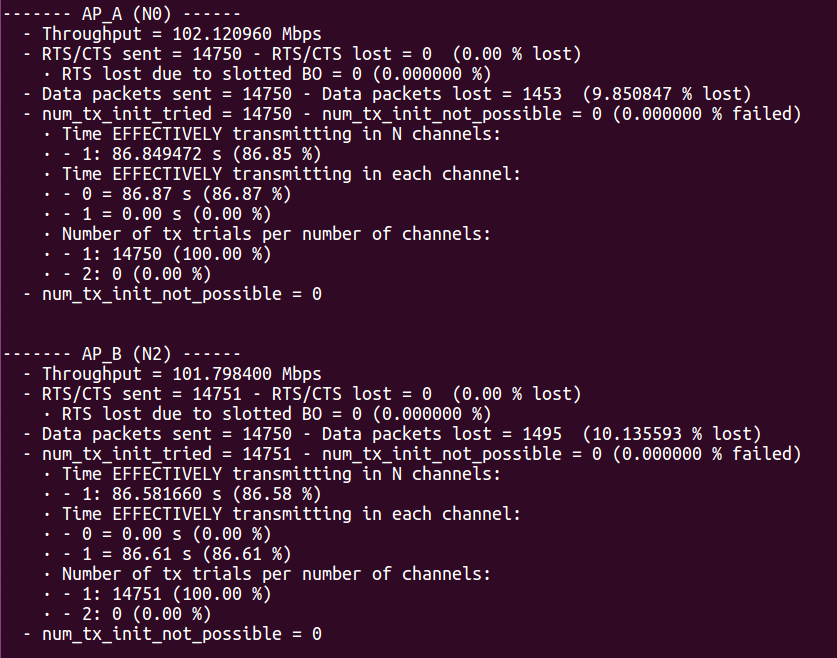
\epsfig{file=images/nodes_statistics_example, width=12cm}
			\caption{Example of nodes statistics in Komondor}
			\label{fig:nodes_statistics_example}
		\end{figure}
		
		\begin{figure}[h!]
			\centering
			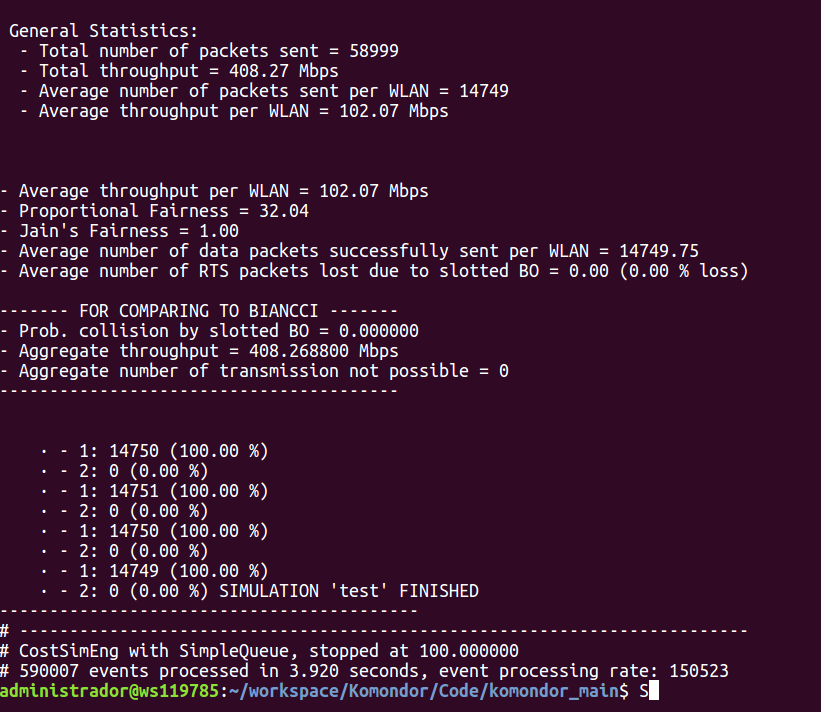
\epsfig{file=images/general_statistics_example, width=12cm}
			\caption{Example of system statistics in Komondor}
			\label{fig:general_statistics_example}
		\end{figure}
	
		% Logs system
		\subsubsection{Events Categorization}
		\label{section:events_categorization}	
		In order to make output results more understandable, logs are categorized according to the event that generates it. With that, further filtering processes can be carried out by developers. Table \ref{table:event_coding} describes the codes used for each type of event.		
		% Events coding table
		\begin{table}[h!]
		\centering
		\scriptsize
		\begin{tabular}{|c|c|c|c|}
		\hline
		\textbf{Method}                            & \textbf{Type}       & \textbf{Sub-type} & \textbf{Event description}                              \\ \hline
		Setup()                                    & A                   & -                 & -                                                       \\ \hline
		\multirow{3}{*}{Start()}                   & \multirow{3}{*}{B}  & B00               & Start()                                                 \\ \cline{3-4} 
		                                           &                     & B01               & Start() end                                             \\ \cline{3-4} 
		                                           &                     & B02               & Node's info (one line)                                  \\ \hline
		\multirow{6}{*}{Stop()}                    & \multirow{6}{*}{C}  & C00               & Stop()                                                  \\ \cline{3-4} 
		                                           &                     & C01               & Stop() end                                              \\ \cline{3-4} 
		                                           &                     & C02               & Time transmitting in number of channels                 \\ \cline{3-4} 
		                                           &                     & C03               & Time transmitting in each channel                       \\ \cline{3-4} 
		                                           &                     & C04               & Packets sent                                            \\ \cline{3-4} 
		                                           &                     & C05               & Throughput                                              \\ \hline
		\multirow{14}{*}{inportSomeNodeStartTX()}  & \multirow{14}{*}{D} & D00               & inportSomeNodeStartTX()                                 \\ \cline{3-4} 
		                                           &                     & D01               & inportSomeNodeStartTX() end                             \\ \cline{3-4} 
		                                           &                     & D02               & Node N has started a TX in channels: c\_left - c\_right \\ \cline{3-4} 
		                                           &                     & D03               & Pre update channel state                                \\ \cline{3-4} 
		                                           &                     & D04               & Distance to transmitting node                           \\ \cline{3-4} 
		                                           &                     & D05               & Power received from transmitting node                   \\ \cline{3-4} 
		                                           &                     & D06               & Post update channel state                               \\ \cline{3-4} 
		                                           &                     & D07               & I am (or not) the TX destination                        \\ \cline{3-4} 
		                                           &                     & D08               & Current SINR                                            \\ \cline{3-4} 
		                                           &                     & D09               & Capacitiy                                               \\ \cline{3-4} 
		                                           &                     & D10               & Primary channel affected (or not)                       \\ \cline{3-4} 
		                                           &                     & D11               & Power sensed in primary channel                         \\ \cline{3-4} 
		                                           &                     & D12               & CCA exceeded (or not)                                   \\ \cline{3-4} 
		                                           &                     & D13               & Backoof active (or not)                                 \\ \hline
		\multirow{10}{*}{inportSomeNodeFinishTX()} & \multirow{10}{*}{E} & E00               & inportSomeNodeFinishTX()                                \\ \cline{3-4} 
		                                           &                     & E01               & inportSomeNodeFinishTX() end                            \\ \cline{3-4} 
		                                           &                     & E02               & N\%d has finished a TX in channel range: \%d - \%d      \\ \cline{3-4} 
		                                           &                     & E03               & Initial power of transmitter                            \\ \cline{3-4} 
		                                           &                     & E04               & Pre update channel state                                \\ \cline{3-4} 
		                                           &                     & E05               & Post update channel state                               \\ \cline{3-4} 
		                                           &                     & E06               & Primary channel affected (or not)                       \\ \cline{3-4} 
		                                           &                     & E07               & Power sensed in primary channel                         \\ \cline{3-4} 
		                                           &                     & E08               & CCA exceeded (or not)                                   \\ \cline{3-4} 
		                                           &                     & E09               & I am transmitting (or not)                              \\ \hline
		\multirow{6}{*}{endBackoff()}              & \multirow{6}{*}{F}  & F00               & endBackoff()                                            \\ \cline{3-4} 
		                                           &                     & F01               & endBackoff() end                                        \\ \cline{3-4} 
		                                           &                     & F02               & Channels for transmitting                               \\ \cline{3-4} 
		                                           &                     & F03               & Transmission is possible (or not)                       \\ \cline{3-4} 
		                                           &                     & F04               & Selected transmission range                             \\ \cline{3-4} 
		                                           &                     & F05               & New backoff generated                                   \\ \hline
		\multirow{3}{*}{myTXFinished()}            & \multirow{3}{*}{G}  & G00               & myTXFinished()                                          \\ \cline{3-4} 
		                                           &                     & G01               & myTXFinished() end                                      \\ \cline{3-4} 
		                                           &                     & G02               & New backoff generated                                   \\ \hline
		\end{tabular}
		\caption{Node's event logs encoding}
		\label{table:event_coding}
		\end{table}

	%%% Code Development
	\subsection{Code development}
	\label{section:code_development}		
	Here we provide some clarifications regarding code implementation, wit the aim to facilitate the Komondor's usage and manipulation to developers that may be interested.
	
		% Considerations
		\subsubsection{Main considerations}
		\label{section:development_considerations}
		% TODO: Extend this part.
		Some technical information regarding code development is worth to be mentioned to properly understand how to use and modify the Komondor simulator. So far, the main considerations to be taken into account are:		
		\begin{itemize}
		\item \textbf{Power and CCA}: power variables are stored in pW (pico watts) in order to be able to operate power magnitudes without loosing resolution\footnote{For instance., the sum of two signals of power values -85 dBm (3.162 pW) and -90 dBm (1 pW), respectively, is -83.803 dBm (4.162 pW).}. However, values are presented to the user in dBm.		
		W (-30)  - mW (0)  - uW (+30) - nW (+60) - pW (+90)\\
		$P_{\text{pw}} = 10^{\frac{P_{\text{dBm}} + 90}{10}}$
		\end{itemize}
	
		% Miscellany
		\subsubsection{Miscellaneous}
		\label{section:development_miscellany}
		% TODO: Extend this part.
			\begin{itemize}
			\item \textbf{Transmitting capability}: we have added a flag to each node that determines if it is able to transmit (1) or not (0), so that we can decide if the node is only listening or both transmitting and listening.
			\item \textbf{Progress bar}: the Komondor simulation progress bar is displayed through a \textit{printf()} command called by any node with \textit{node\_id} set to 0. If no node has \textit{node\_id} set to 0, the progress bar is not displayed.
			\end{itemize}
	
%%%%%%%%%%%%%%%
% 6. CONCLUSIONS
%%%%%%%%%%%%%%%
\section{Conclusions}
\label{section:conclusions}
In this document we provided an overview of the first version of the Komondor simulator, which aims to reproduce the basic operation of IEEE 802.11ax WLANs in addition to allow the utilization of intelligent systems. We introduced the system model considered when building the simulator, as well as the main MAC features implemented. Additionally, due to the open source nature of this project, we provided basic information of interest for developers that are expected to use or even modify this HD WLANs simulator.

Regarding the validation of the simulator, we provided a set of meaningful test scenarios to prove the proper behavior of the simulator. As shown, tests were satisfactory as the throughput computed with Komondor and the CTMN model are pretty similar, and the differences were properly justified.

This project is expected to move forward for including of novel mechanisms such as OFDMA, MU-MIMO, TPC or  CST adjustment. In addition, intelligent agents are expected to be included for making operations such as Dynamic CB (DCB).

%%% BIBLIOGRAPHY
\bibliographystyle{unsrt}
\bibliography{bib}

\end{document}